% Chapter 4 from the standard thesis template
%   that contains an adv. example table and figure.
\chapter{TESTING AND VERIFICATION}

Testing and verification ensures that the new components that we have added to the system are working as intended and has not caused a negative impact on the overall system performance.  To do this, several tests were conducted and verification was obtained by using a well known method of detecting power in a radiometer, a square-law detector.  

Testing began with the square-law detector as this was one of the first components that was obtained.  Next, testing was done with the the software defined radio as a whole.  Further testing was done including a test run of the system and was used in the Dr. Brian Hornbuckle's E E 518 class.  Finally a cold bath test was done with both the software defined radio and with the square law detector as a system to verify both functionality and to compare the results from both devices.  

\section{Square-law Detector}
To verify the results that the software defined radio is obtaining, a square-law detector is used to measure the power of the incoming signal.  The incoming signal is split using a power divider so that the signal will be the same to both devices with the exception of the 3 dB plus insertion loss the power divider adds.  This allows us to verify the software defined radio with a proven system.  Square-law detectors have traditionally been used in radiometers and have been proven to work in radiometer applications.  They are also a very simple device which means there is little that can go wrong with using them.


\subsection{Analog Devices ADL5902}

The square-law detector that we obtained is the Analog Devices ADL5902.  The ADL5902 is a true rms responding power detector that has a square law detector, a variable gain amplifier and an output driver. It also has a temperature sensor and will compensate for temperature variations.  The output driver allows for the small signal from the square law detector to be amplified to a level that most analog to digital devices can detect.  This driver however does have low noise and has a noise output of approximately $25nV/ \sqrt{Hz}$ at 100 kHz.  The ADL5902 operates from 50 MHz to 9 GHz and in most cases can detect down to $-60$ dBm.  This works well in our application since the radiometer operates at 1.4 GHz and after the amplification stage we usually see between $-40$ to $-30$ dBm of power.  

The specifications of the ADL5902 can be seen in Table~\ref{data}
shown below.

\begin{table}[h!tb] \centering
\isucaption{ADL5902 Specifications}
\label{data}
% Use: \begin{tabular{|lcc|} to put table in a box
\begin{tabular}{lcc} \hline
\textbf{Parameter @ 900 MHz} & \textbf{Value} & \textbf{Units} \\ \hline
Frequency Range & 50 to 9000 & MHz \\
Dynamic Range & 61 & dB \\
Minimum Input Level, $\pm 1.0$ dB & 60 & dB \\ 
Maximum Input Level, $\pm 1.0$ dB & 1 & db \\
Logarithmic Slope & 53.7 & mV/dB \\ 
Output Voltage Range & 0.03 to 4.8 & V \\ \hline
\end{tabular}
\end{table}

The ADL5902 outputs an analog signal that falls between 0.03 volts and 4.8 volts.  It outputs a change of 53.7 millivolt per dB detected by the ADL5902.  

%\subsubsection{Parts of the hypothesis}

%Here one particular part of the hypothesis that is 
%currently being explained is examined and particular
%elements of that part are given careful scrutiny.

% Below \subsubsection
% Sectional commands: \paragraph and \subparagraph may also be used

\subsection{Data acquisition and storage}

In order to analyze the data, a method was developed to acquire the data and store it for later use.  For the N200 software defined radio, this is done automatically by the GNURadio program.  Both the complete signal and the power information is stored to a file for later analysis.  The square-law detector however outputs information as an analot voltage that is linearly proportional to the RF power measured.  This required a system that can capture the analog signal from the ADL5902 and then send the data to be stored.  This was done using a PIC32 processor, specifically the PIC32MX795F512L processor which has a 10-bit analog to digital converter built in.  To aid in rapid development of the system, a BitWhacker board purchased through Sparkfun was used.  Once the data was captured by the A/D converter, the PIC32 processor then sent this information through a RS232 port which can then be read by a computer.  The computer would then store this information to a file.  While it is certainly possible for the PIC32 to store this information to a SD card or other external memory device, the computer was used so that it would be possible to synchronize the data with the data being send from the SDR.

\subsubsection{PIC32 Micro-controller system}

The PIC32MX795F512L is the processor that was selected to acquire the analog voltage the ADL5902 outputs.  This processor was chosen for the reason that it would allow for additional radiometer functions to be added to it later.  The ISU radiometer currently uses a Rabbit based micro-controller.  However, it was soon discovered that this processor was not able to handle all the tasks given to it efficiently.  A new micro-controller system was known to be needed and thus this processor was chosen to handle not only the task for of obtaining information from the square-law detector but would have plenty of room for doing other tasks needed in the ISU radiometer. 

The ISU radiometer has several analog temperature sensors and two thermal electric coolers (TEC) that also need to be monitored and controlled.  In addition, control lines are needed to control the RF switches within the radiometer as well turning on and off the noise diode source.  The TECs used in the ISU radiometer require a RS232 serial connection.  In addition, it was also known that a GPS unit would also be added.  This meant that at least 4 RS232 ports were needed including sending the data from the square-law detector.  The micro-controller would also need to monitor at least 6 analog temperature sensors that are found at various points within the ISU radiometer.  These requirements combined with the ability to add future sensors and/or tasks to the micro-controller led us to select this processor.

For the testing that was conducted for this thesis work, the PIC32MX795F512L is setup to capture the analog signal from the square-law detector using one of the 10-bit analog to digital ports it has.  This information is then sent through one of the PIC32MX795F512L UART ports so that it can be read by the host computer.


\subsection{Tests on the ADL5902}
To test the ADL5902 a signal generator was used that had a controlled output.  The specific signal generator that was used was an older model that allowed us to change the output in 10 dBm increments.  The signal generator was also configured for 1.4 GHz as that is the frequency the ISU radiometer is configured to listen at.  Ideally a noise generator would have been desirable, however a noise generator with adjustable power output could not be located on campus.  

The ADL5902 is available from Analog Devices in an evaluation board.  This board pairs the ADL5902 with a AD7466 12-bit analog to digital converter.  This board can then be mated with Analog Devices BlackFin processor which acts as a USB gateway for the AD7466 data.  A test program written in LabView is also provided as well.

The test program provided by Analog Devices allows us to query the ADL5902 and record the raw ADC value.  The test program also allows us to enter in the frequency used during testing and the temperature during the test.  The test program also allows us to calibrate the system as well.  All of the data is then stored into an Excel spreadsheet which can be accessed later.

For this test we used the signal generator set to 1.4 GHz and started at $-60$ dBm for the output signal.  This was selected as this is the lowest the square law detector can detect.  The output power was then incremented on the signal generator in 10 dBm steps.  There was no change to any other parameter.  This was done up to 0 dBm.  Any higher and there was risk of damage to the ADL5902.  This test was then repeated several times and was done with the signal generator stepping up from $-60$ dBm to 0 dBm and from 0 dBm to $-60$ dBm.  

The data collected was then graphed using Excel.  The graph shown in~\ref{adl5902}
Shows that the ADL5902 has a linear output and matches the expected value based on the input.  

\begin{figure}[h!tb] \centering

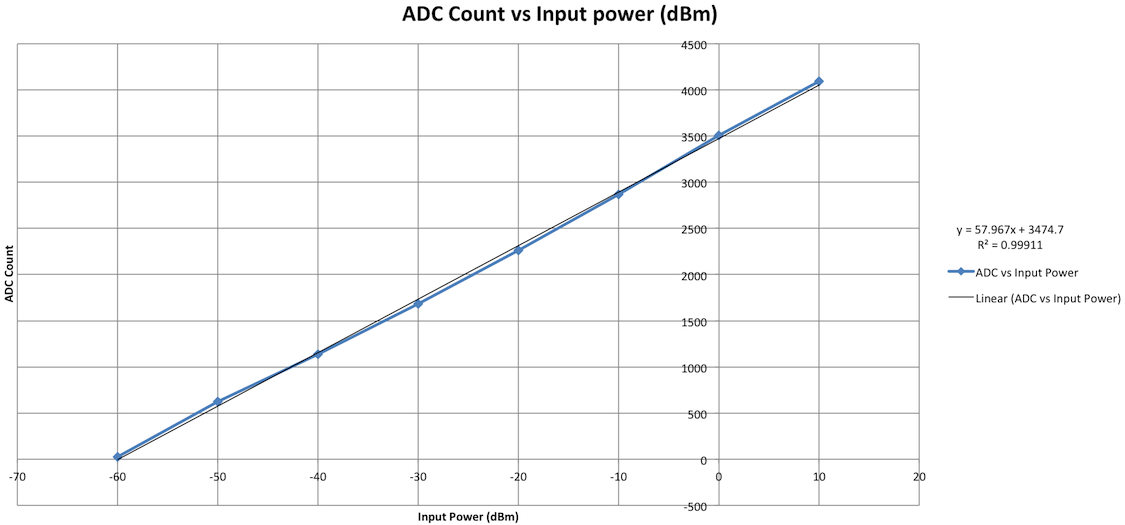
\includegraphics[width=\textwidth]{Images/Linearsquarelaw}

\isucaption{Graph showing the linearity of the ADL5902}
\label{adl5902}
\end{figure}

The ADL5902 test board was considered to be used in the final design for the ISU radiometer and in additional tests.  However, Analog Devices decided to make the information to communicate with the BlackFin processor proprietary and this hampered attempts to integrate that system into our overall system design.  For this reason, it was decided to simply record the analog data that the ADL5902 itself puts out and the PIC32 described above was used to capture and send this information.

\section{Software Defined Radio tests}
Once it was confirmed that the square-law detector was working within the specifications that were given, testing then moved to the software defined radio.  Once the Python program was established for replicating a total power radiometer in software, this was then loaded into GNURadio and used to control the N200 SDR.  GNURadio has a built in noise generator that was then used to test the program and it's ability to measure small changes in noise.  This simulated noise verified that the program written was able to detect changes in noise power using a simulated Gaussian source.  It was desired to also use a hardware based noise generator, however a suitable noise generator could not be located on campus.

\section{E E 518 Lab Tests}

Further testing of the square-law detector was performed by using the radiometer in a real world event.  This test was exercised in conjunction with the Microwave Remote Sensing class (E E 518) under Dr. Brian Hornbuckle.  For this test the radiometer was installed on the roof of Agronomy Hall and was configured so that it could be rotated so it will have a clear view of the sky.  This allowed us to make measurements with a cold source and then at the ground to record a warm source.


{\begin{figure}[h!tb] 
\centering
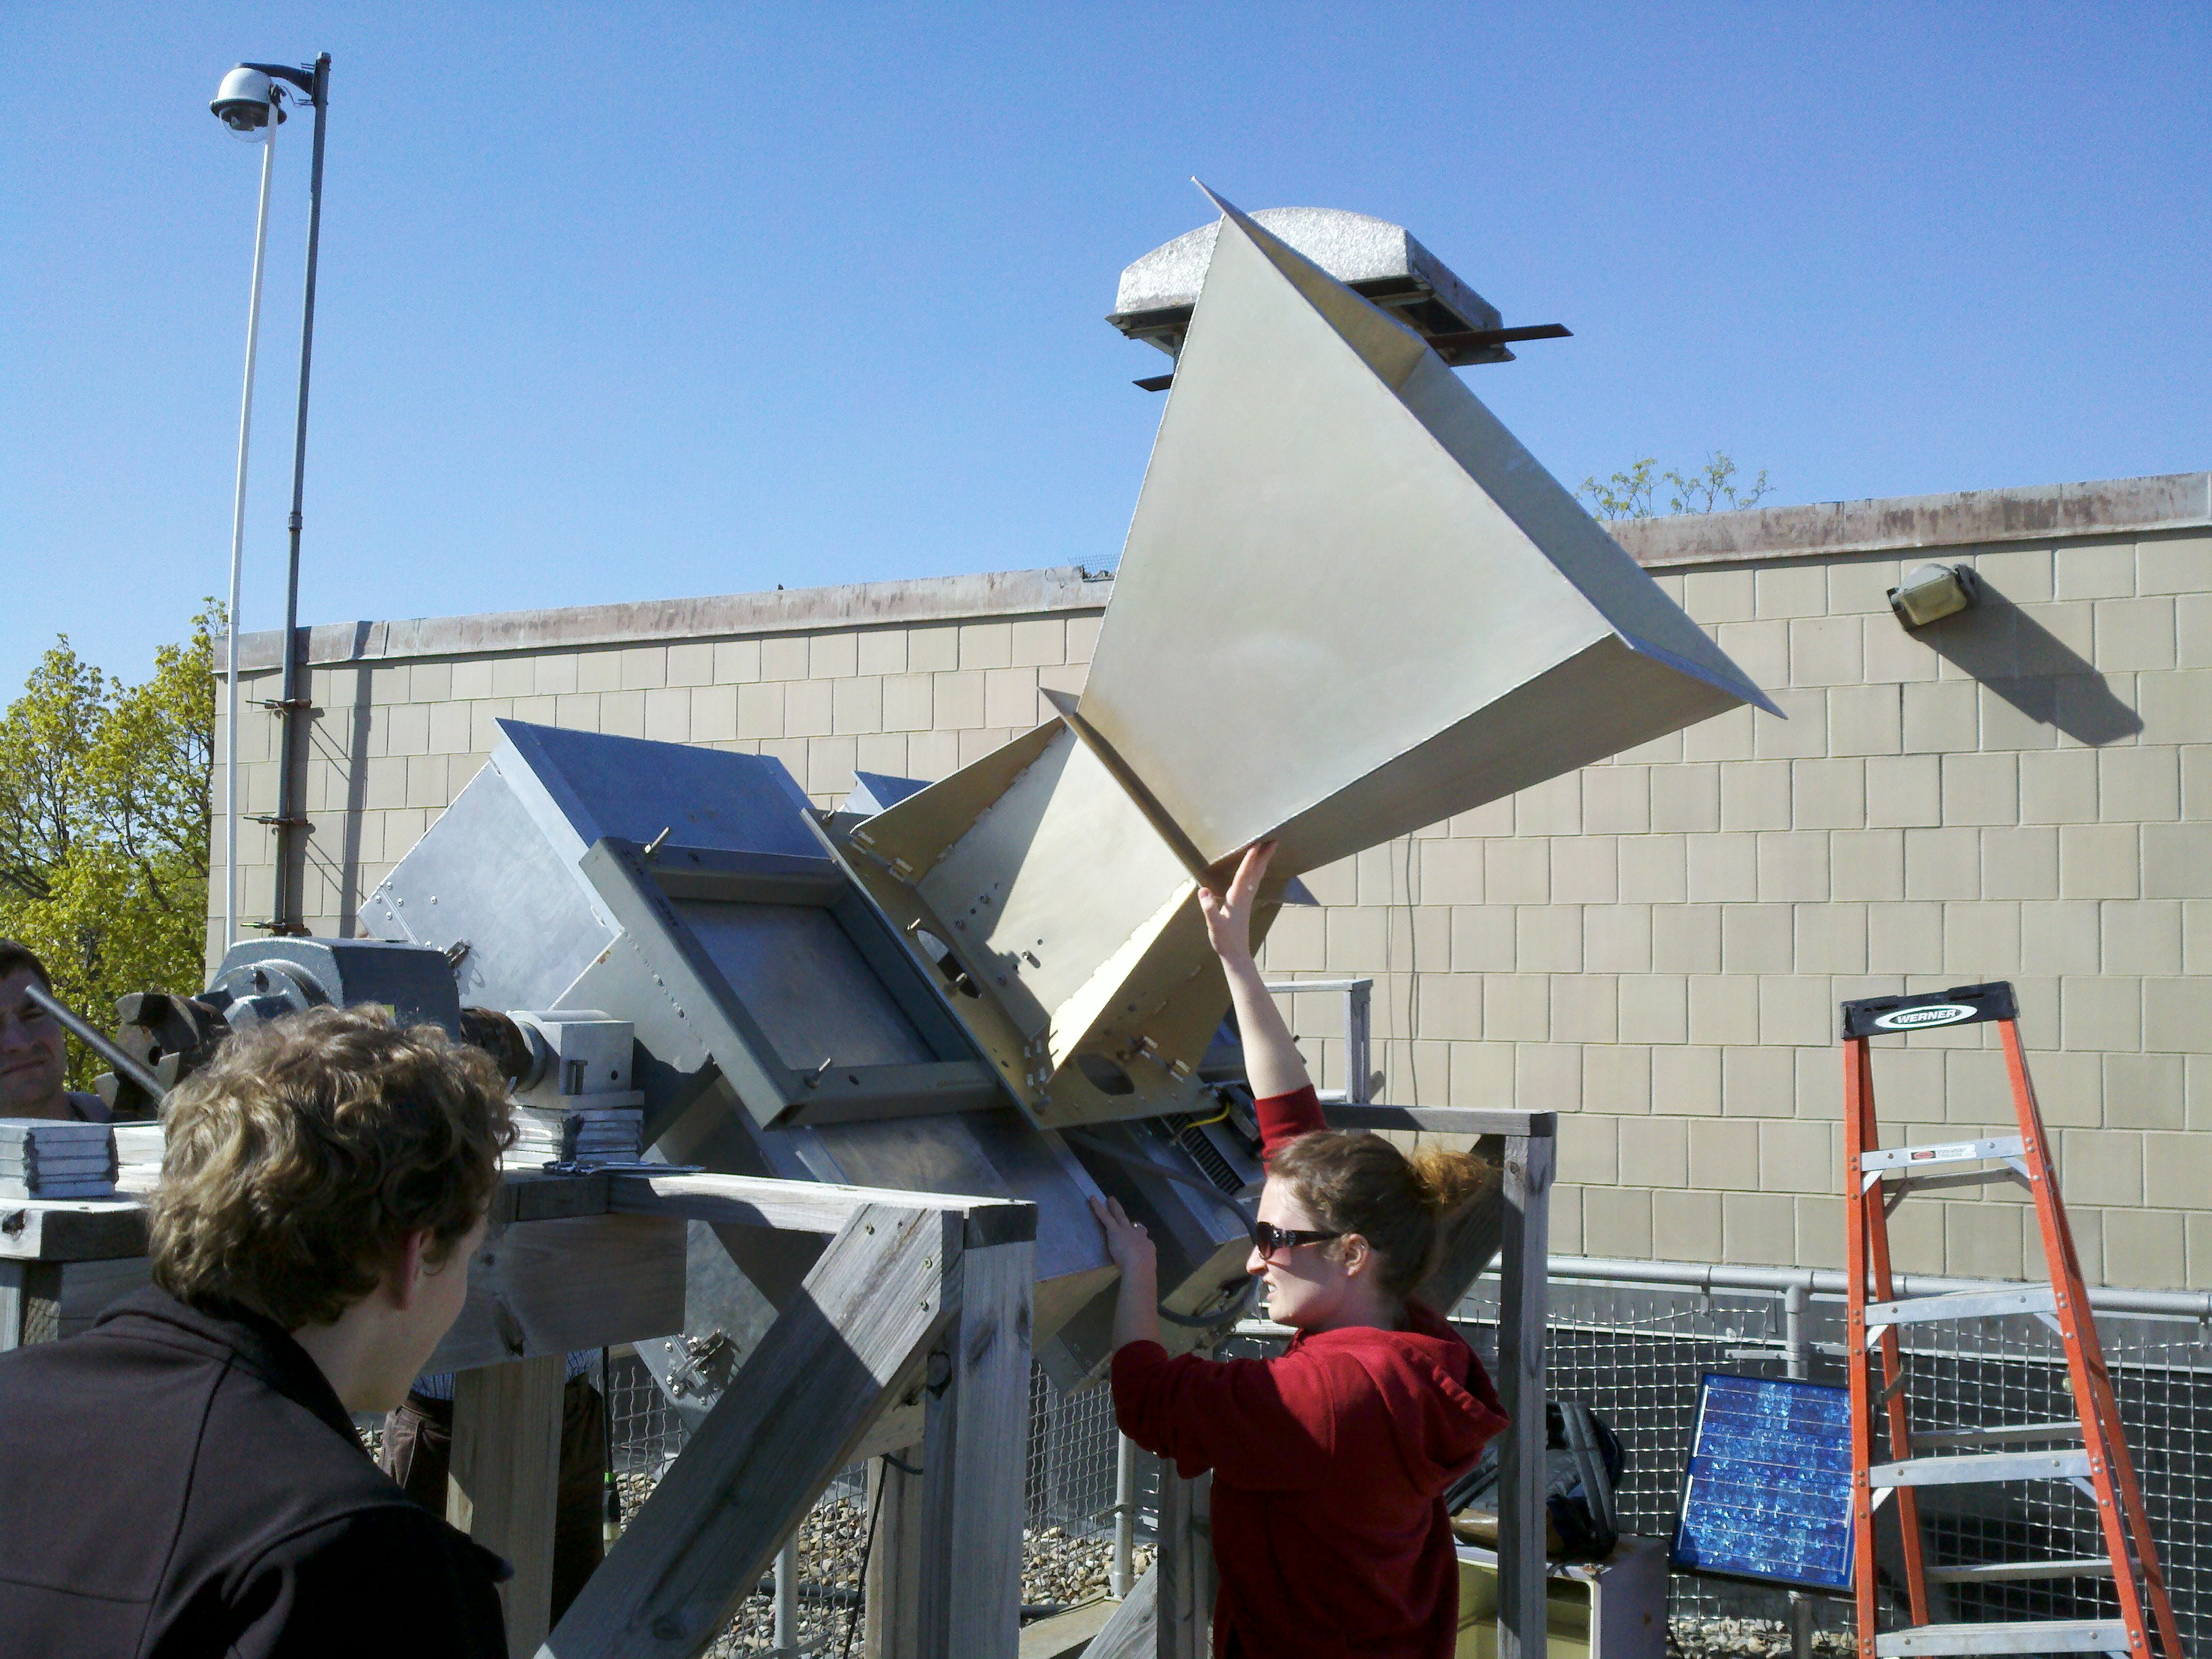
\includegraphics[width=\textwidth]{Images/radiometer_roof.jpg}
\isucaption{Students rotating the radiometer for an experiment on Agronomy Hall}
\label{radiometer_roof}
\end{figure}
}

\section{Total Power Radiometer Test with Cold Water Bath}
To fully test both the total power radiometer in the software defined radio and the square-law detector, a cold water bath experiment was established to verify that both the square-law detector and SDR was able to measure real world changes in the noise.  In addition, this would also give us a calibration test (confirm this) line to work with.

\subsection{Laboratory Setup}
For this experiment the, ISU radiometer was setup in a laboratory that had access to measurement tools.  To measure the change in noise, a 50 ohm load was attached to the radiometer.  The ISU radiometer, with the current filters and LNAs would then amplify and filter the signal.  This signal was then measured by the square-law detector and the N200 SDR.  The 50 ohm load was then submersed into a hot or cold bath.  These water baths were temperature controlled for 100 degrees Centigrade and to 10 degrees Centigrade.  The load was submersed in each bath for 2 minutes to allow for it to reach the same temperature as the bath.  The noise measured was then recorded using GNURadio with the N200 SDR or with the PIC32 setup on the square-law detector.  In addition to the total power measurements, the raw I-Q data was also recorded.  This allowed us to replay the experiment through GNURadio for further study.
\subsection{Test Results}

Several experiments were conducted with this cold-bath configuration to establish that the results were reproducible.  In each case, the experiment showed that both the square-law detector and the SDR were able to measure a change of noise temperature.  Once experiment used a change of only 50 C and the change was easily recorded on the SDR.  Using the experiment described in which the temperatures were held constant, this also gave us a calibration point that we can use to calibrate the radiometer.

\section{Liquid Nitrogen Test}
The Liquid Nitrogen Test was conducted to verify that the radiometer was able to operate within the specifications that were given for the radiometer.  This test is also a fairly common test for testing and calibrating a traditional type of radiometer.  With this test, we can test the radiometer by measuring extreme values for the noise temperature.  To do this, we submerge a matched load attached to the radiometer into a liquid nitrogen bath.  This cools the load, which represents our source, to a physical temperature of approximately 77 Kelvin.  We can then select several "warmer" temperatures such as a ice water bath, room temperature or even boiling water.  Since we expect that the radiometer is linear in how it responds to these noise temperatures, we can then build a calibration line for the radiometer.

\subsection{Testing Apparatus}
To run this test, we need to have some equipment for this.  First and foremost, we need a radiometer.  For this test we used the ISU Radiometer front end, with the LNAs and bandpass filters in place.  The noise diode was turned off for these experiments.  A fifty ohm matched load was then attached to low loss coax and represented our source to the radiometer.  Finally, the output of the radiometer was run to the Ettus N200 software defined radio instead of running the on-board Analog to Digital converter and FPGA.  The data from the N200 was then sent to a MacBook Pro running GNURadio and the custom software that I had written.  This data is sent to the MacBook Pro through a 1 gigabit Ethernet connection due to the large bandwidth coming from the N200.  For these experiments, we only used one "side" of the radiometer.  In theory, both sides of the ISU radiometer should be identical as far as results go.
\subsection{Test Run 1}

\section{Further testing}